\documentclass[tikz,border=10pt]{standalone}
\usetikzlibrary{matrix, arrows.meta, positioning, calc, fit}
\usepackage{amssymb, amsmath}

\begin{document}
	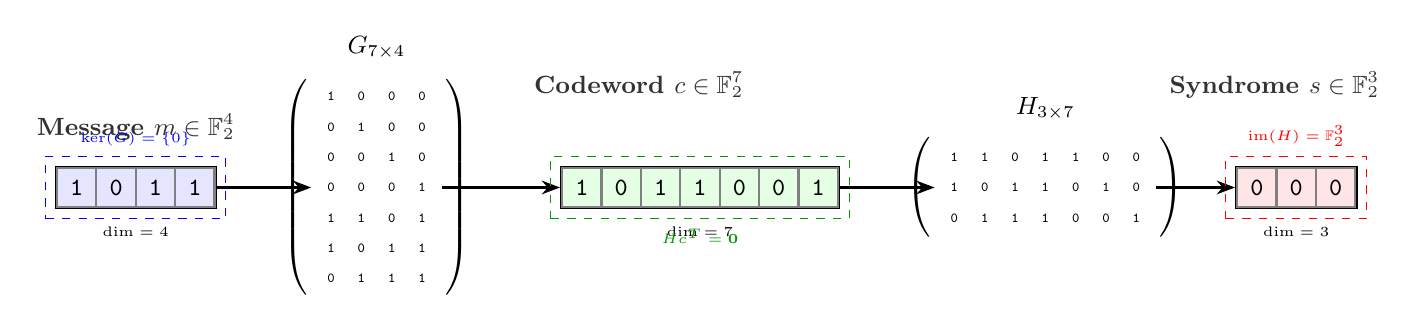
\begin{tikzpicture}[
		font=\sffamily,
		% Style for the bit-vector registers
		bitvector/.style={
			matrix of nodes,
			nodes={draw=black!50, minimum size=5mm, anchor=center, font=\ttfamily\small},
			column sep=-\pgflinewidth,
			row sep=-\pgflinewidth,
			inner sep=0pt,
			draw=black, thick
		},
		% Style for the Operator Matrices (G and H)
		opmatrix/.style={
			matrix of nodes,
			nodes={font=\ttfamily\tiny, minimum size=3.5mm, anchor=center},
			left delimiter=(, right delimiter=),
			column sep=1pt, row sep=1pt,
			inner sep=2pt
		},
		labelnode/.style={font=\bfseries\small, color=black!80}
		]
		
		% --- 1. MESSAGE SPACE (F2^k) ---
		\node[labelnode] (L1) at (0, 2) {Message $m \in \mathbb{F}_2^4$};
		\matrix (m) [bitvector, below=0.2cm of L1, fill=blue!10] {
			1 & 0 & 1 & 1 \\
		};
		\node[below=0.1cm of m, font=\tiny] {$\text{dim}=4$};
		
		% --- 2. GENERATOR TRANSFORMATION (G) ---
		\matrix (G) [opmatrix, right=1.2cm of m] {
			1 & 0 & 0 & 0 \\
			0 & 1 & 0 & 0 \\
			0 & 0 & 1 & 0 \\
			0 & 0 & 0 & 1 \\
			1 & 1 & 0 & 1 \\
			1 & 0 & 1 & 1 \\
			0 & 1 & 1 & 1 \\
		};
		\node[above=0.1cm of G, font=\small\itshape] {$G_{7 \times 4}$};
		
		% --- 3. AMBIENT SPACE (F2^n) ---
		\node[labelnode] (L2) at ($(G.east) + (2.5, 1.3)$) {Codeword $c \in \mathbb{F}_2^7$};
		\matrix (c) [bitvector, right=1.5cm of G, fill=green!10] {
			1 & 0 & 1 & 1 & 0 & 0 & 1 \\
		};
		\node[below=0.1cm of c, font=\tiny] {$\text{dim}=7$};
		
		% --- 4. PARITY CHECK TRANSFORMATION (H) ---
		\matrix (H) [opmatrix, right=1.2cm of c] {
			1 & 1 & 0 & 1 & 1 & 0 & 0 \\
			1 & 0 & 1 & 1 & 0 & 1 & 0 \\
			0 & 1 & 1 & 1 & 0 & 0 & 1 \\
		};
		\node[above=0.1cm of H, font=\small\itshape] {$H_{3 \times 7}$};
		
		% --- 5. SYNDROME SPACE (F2^{n-k}) ---
		\node[labelnode] (L3) at ($(H.east) + (1.5, 1.3)$) {Syndrome $s \in \mathbb{F}_2^3$};
		\matrix (s) [bitvector, right=1cm of H, fill=red!10] {
			0 & 0 & 0 \\
		};
		\node[below=0.1cm of s, font=\tiny] {$\text{dim}=3$};
		
		% --- ARROWS & FLOW ---
		\draw[-Stealth, thick] (m.east) -- (G.west);
		\draw[-Stealth, thick] (G.east) -- (c.west);
		\draw[-Stealth, thick] (c.east) -- (H.west);
		\draw[-Stealth, thick] (H.east) -- (s.west);
		
		% --- ANNOTATIONS FOR EXACTNESS ---
		% Exactness at Fk (Injectivity)
		\node[draw=blue, dashed, fit=(m), label={[blue, font=\tiny]above:$\ker(G)=\{0\}$}] {};
		
		% Exactness at Fn (im G = ker H)
		\node[draw=green!60!black, dashed, fit=(c), label={[green!60!black, font=\tiny]below:$Hc^T = \mathbf{0}$}] {};
		
		% Exactness at Fnk (Surjectivity)
		\node[draw=red, dashed, fit=(s), label={[red, font=\tiny]above:$\text{im}(H) = \mathbb{F}_2^3$}] {};
		
	\end{tikzpicture}
\end{document}